\clearpage
\setcounter{page}{1}
\maketitlesupplementary


\section{Embodied Joint Codebook Mapping Table}

As introduced in Section 3.3.2 of the main paper, the Embodied Joint Codebook is central to our structural-centric formulation, enabling the policy to handle morphological heterogeneity. It resolves the ambiguity of our unordered, variable-length action sequence $\mathbf{A}_t \in \mathbb{R}^{D_a \times T}$ by providing a unique, learnable embedding for each joint. Table \ref{tab:codebook_mapping} provides the mapping used in our experiments.







\section{3D Re-implementation of HPT and UniAct}

To ensure a fair and rigorous comparison against our 3D-native approach, we adapt the primary 2D-based baselines, HPT \cite{wang2024scaling} and UniAct \cite{zheng2025universal}, to accept 3D point cloud inputs. This adaptation is crucial as these models, in their original form, cannot process the 3D observation space used by SAT. Results are presented in Table~\ref{tab:app_3dhpt_uniact}.


\subsection{3D-HPT}
The HPT \cite{wang2024scaling} framework is designed with a modality-specific ``stem'' and a shared ``trunk'' transformer. The original model employs 2D vision stems to process image-based inputs. For our 3D baseline (referred to as 3D-HPT), we replace the original 2D vision stem with a 3D-specific stem. This new stem is architected similarly to our own observation tokenizer (Section 3.3.1), utilizing a hierarchical PointNet-based encoder. It processes the raw point cloud $\mathcal{P}_t$ by performing Farthest Point Sampling (FPS) and K-Nearest Neighbor (KNN) grouping to extract local geometric tokens, along with a global scene token. These 3D tokens are then projected to the required embedding dimension and fed into the original, unchanged HPT trunk. This modification allows HPT to leverage 3D geometric information while maintaining the integrity of its core architecture.

\subsection{3D-UniAct}
The adaptation of UniAct \cite{zheng2025universal} requires a different approach, as its architecture is deeply integrated with a Vision-Language Model (VLM). The core VLM-based component, which processes sequences of discretized tokens, is left unmodified. Our intervention focuses on the visual tokenizer and re-encoding stages. The original UniAct feeds visual tokens, generated by a 2D tokenizer, into the VLM. Crucially, it also re-introduces raw visual features at later stages to ground the policy's output. We replace this second, ``in-the-loop'' 2D feature encoder with a 3D PointNet encoder. This 3D encoder takes the raw point cloud $\mathcal{P}_t$ as input at each relevant time step, processes it, and provides the necessary 3D-grounded visual conditioning to the policy decoder. This allows the model to operate on 3D data while retaining its original reasoning and action-generation mechanism.

\begin{table*}[t]
\centering
\small
\resizebox{0.90\textwidth}{!}{
\begin{tabular}{l|c|c|c|c|c}
\toprule
  % & & \multicolumn{3}{c|}{Simulation Benchmark (\# tasks)} & \\
  Method & Modality & Adroit (3)~\cite{rajeswaran2017learning} & DexArt (4)~\cite{bao2023dexart} & Bi-DexHands (4)~\cite{chen2023bi} & Average Success  \\
\midrule
  3D-HPT~\cite{wang2024scaling} & 3D & \dd{0.50}{0.02}  & \dd{0.55}{0.05} & \dd{0.49}{0.04} & \dd{0.51}{0.04}  \\
  3D-UniAct~\cite{zheng2025universal} & 3D & \dd{0.50}{0.01} & \dd{0.55}{0.03} & \dd{0.49}{0.07} & \dd{0.51}{0.05} \\

  \textbf{\mymethod{} (Ours)} & 3D & \ddbfgreen{0.75}{0.02} & \ddbfgreen{0.73}{0.03} & \ddbfgreen{0.67}{0.05} & \ddbfgreen{0.71}{0.04} \\
\bottomrule
\end{tabular}
}
% \vspace{-8pt}
\caption{Quantitative comparison of our method against 3D re-implementation of HPT~\cite{wang2024scaling} and UniAct~\cite{zheng2025universal} on 11 dexterous manipulation tasks from the Adroit~\cite{rajeswaran2017learning}, DexArt~\cite{bao2023dexart}, and Bi-DexHands~\cite{chen2023bi} simulation benchmarks.}
% \vspace{-16pt}
\label{tab:app_3dhpt_uniact}
\end{table*}

\begin{table}[t]
\centering
\small
\resizebox{0.46\textwidth}{!}{
\begin{tabular}{c|cc|c}
\toprule
Horizon Length $T$ & Average Success on Adroit (3) \\
\midrule
8 & \dd{0.51}{0.03} \\
16 & \ddbfgreen{0.54}{0.02} \\
32 & \dd{0.47}{0.03} \\
64 & \dd{0.43}{0.04} \\
\bottomrule
\end{tabular}
}
% \vspace{-8pt}
\caption{Ablation on action horizon length $T$.}
% \vspace{-16pt}
\label{tab:app_horizon}
\end{table}

\begin{figure}[t]
  \centering
  \includegraphics[width=0.96\linewidth]{pic/app_fail.pdf}
  % \vspace{-16pt}
  \caption{Failure case analysis.}
  % \vspace{-16pt}
  \label{fig:failure_cases}
\end{figure}

\begin{table*}[t]
    \centering
    \caption{Embodied Joint Codebook mapping for manipulators used in pre-training and evaluation. The indices for Functional Category and Rotation Axis are shared across all embodiments, forming the basis for cross-embodiment skill transfer. (To be continued ...)}
    \label{tab:codebook_mapping}
    \resizebox{0.99\textwidth}{!}{
    \begin{tabular}{llccc}
        \toprule
        \textbf{Embodiment} & \textbf{Joint Name} & \textbf{Embodiment ID ($e$)} & \textbf{Functional Category ($f$)} & \textbf{Rotation Axis ($r$)} \\
        \midrule
        \textbf{Shadow Dexterous Hand} & T-CMC & 1 & 1 (CMC) & 1 (Flexion/Extension) \\
         & T-CMC & 1 & 1 (CMC) & 2 (Abduction/Adduction) \\
         & T-CMC & 1 & 1 (CMC) & 3 (Rotation) \\
         & T-MCP & 1 & 2 (MCP) & 1 (Flexion/Extension) \\
         & T-IP & 1 & 3 (PIP) & 1 (Flexion/Extension) \\
         & IF-CMC & 1 & 1 (CMC) & 1 (Flexion/Extension) \\
         & IF-CMC & 1 & 1 (CMC) & 2 (Abduction/Adduction) \\
         & IF-CMC & 1 & 1 (CMC) & 3 (Rotation) \\
         & IF-MCP & 1 & 2 (MCP) & 1 (Flexion/Extension) \\
         & IF-MCP & 1 & 2 (MCP) & 2 (Abduction/Adduction) \\
         & IF-MCP & 1 & 2 (MCP) & 3 (Rotation) \\
         & IF-PIP & 1 & 3 (PIP) & 1 (Flexion/Extension) \\
         & IF-DIP & 1 & 4 (DIP) & 1 (Flexion/Extension) \\
         & MF-CMC & 1 & 1 (CMC) & 1 (Flexion/Extension) \\
         & MF-CMC & 1 & 1 (CMC) & 2 (Abduction/Adduction) \\
         & MF-CMC & 1 & 1 (CMC) & 3 (Rotation) \\
         & MF-MCP & 1 & 2 (MCP) & 1 (Flexion/Extension) \\
         & MF-MCP & 1 & 2 (MCP) & 2 (Abduction/Adduction) \\
         & MF-MCP & 1 & 2 (MCP) & 3 (Rotation) \\
         & MF-PIP & 1 & 3 (PIP) & 1 (Flexion/Extension) \\
         & MF-DIP & 1 & 4 (DIP) & 1 (Flexion/Extension) \\
         & RF-CMC & 1 & 1 (CMC) & 1 (Flexion/Extension) \\
         & RF-CMC & 1 & 1 (CMC) & 2 (Abduction/Adduction) \\
         & RF-CMC & 1 & 1 (CMC) & 3 (Rotation) \\
         & RF-MCP & 1 & 2 (MCP) & 1 (Flexion/Extension) \\
        \bottomrule
    \end{tabular}
    }
\end{table*}


% ===================================================================
\begin{table*}[t]
    \ContinuedFloat % 声明这是接续的浮动体
    \centering
    \caption[]{Embodied Joint Codebook mapping... (Continued)} % 续表标题
    \resizebox{0.99\textwidth}{!}{
    \begin{tabular}{llccc}
        \toprule
        \textbf{Embodiment} & \textbf{Joint Name} & \textbf{Embodiment ID ($e$)} & \textbf{Functional Category ($f$)} & \textbf{Rotation Axis ($r$)} \\
        \midrule
        \textbf{Shadow Dexterous Hand} & RF-MCP & 1 & 2 (MCP) & 2 (Abduction/Adduction) \\
         & RF-MCP & 1 & 2 (MCP) & 3 (Rotation) \\
         & RF-PIP & 1 & 3 (PIP) & 1 (Flexion/Extension) \\
         & RF-DIP & 1 & 4 (DIP) & 1 (Flexion/Extension) \\
         & LF-CMC & 1 & 1 (CMC) & 1 (Flexion/Extension) \\
         & LF-CMC & 1 & 1 (CMC) & 2 (Abduction/Adduction) \\
         & LF-CMC & 1 & 1 (CMC) & 3 (Rotation) \\
         & LF-MCP & 1 & 2 (MCP) & 1 (Flexion/Extension) \\
         & LF-MCP & 1 & 2 (MCP) & 2 (Abduction/Adduction) \\
         & LF-MCP & 1 & 2 (MCP) & 3 (Rotation) \\
         & LF-PIP & 1 & 3 (PIP) & 1 (Flexion/Extension) \\
         & LF-DIP & 1 & 4 (DIP) & 1 (Flexion/Extension) \\
        \midrule
        \textbf{SCHUNK SVH Five-Finger Hand} & T-CMC & 3 & 1 (CMC) & 1 (Flexion/Extension) \\
         & T-CMC & 3 & 1 (CMC) & 2 (Abduction/Adduction) \\
         & T-MCP & 3 & 2 (MCP) & 1 (Flexion/Extension) \\
         & T-IP & 3 & 3 (PIP) & 1 (Flexion/Extension) \\
         & IF-MCP & 3 & 2 (MCP) & 1 (Flexion/Extension) \\
         & IF-MCP & 3 & 2 (MCP) & 2 (Abduction/Adduction) \\
         & IF-PIP & 3 & 3 (PIP) & 1 (Flexion/Extension) \\
         & MF-MCP & 3 & 2 (MCP) & 1 (Flexion/Extension) \\
         & MF-MCP & 3 & 2 (MCP) & 2 (Abduction/Adduction) \\
         & MF-PIP & 3 & 3 (PIP) & 1 (Flexion/Extension) \\
         & RF-MCP & 3 & 2 (MCP) & 1 (Flexion/Extension) \\
         & RF-MCP & 3 & 2 (MCP) & 2 (Abduction/Adduction) \\
         & RF-PIP & 3 & 3 (PIP) & 1 (Flexion/Extension) \\
         & LF-MCP & 3 & 2 (MCP) & 1 (Flexion/Extension) \\
         & LF-MCP & 3 & 2 (MCP) & 2 (Abduction/Adduction) \\
         & LF-PIP & 3 & 3 (PIP) & 1 (Flexion/Extension) \\
        \midrule
        \textbf{Tesla Optimus Gen 2 Hand} & T-CMC & 4 & 1 (CMC) & 1 (Flexion/Extension) \\
         & T-CMC & 4 & 1 (CMC) & 2 (Abduction/Adduction) \\
         & T-MCP & 4 & 2 (MCP) & 1 (Flexion/Extension) \\
         & IF-MCP & 4 & 2 (MCP) & 1 (Flexion/Extension) \\
         & IF-PIP & 4 & 3 (PIP) & 1 (Flexion/Extension) \\
         & MF-MCP & 4 & 2 (MCP) & 1 (Flexion/Extension) \\
         & MF-PIP & 4 & 3 (PIP) & 1 (Flexion/Extension) \\
         & RF-MCP & 4 & 2 (MCP) & 1 (Flexion/Extension) \\
         & RF-PIP & 4 & 3 (PIP) & 1 (Flexion/Extension) \\
         & LF-MCP & 4 & 2 (MCP) & 1 (Flexion/Extension) \\
         & LF-PIP & 4 & 3 (PIP) & 1 (Flexion/Extension) \\
        \midrule
        \textbf{Robotiq} & IF-MCP & 5 & 2 (MCP) & 1 (Flexion/Extension) \\
         & IF-PIP & 5 & 3 (PIP) & 1 (Flexion/Extension) \\
         & MF-MCP & 5 & 2 (MCP) & 1 (Flexion/Extension) \\
         & MF-PIP & 5 & 3 (PIP) & 1 (Flexion/Extension) \\
         & LF-MCP & 5 & 2 (MCP) & 1 (Flexion/Extension) \\
         & LF-PIP & 5 & 3 (PIP) & 1 (Flexion/Extension) \\
        \bottomrule
    \end{tabular}
    }
\end{table*}


% ===================================================================
\begin{table*}[t]
    \ContinuedFloat % 声明这是接续的浮动体
    \centering
    \caption[]{Embodied Joint Codebook mapping... (Continued)} % 续表标题
    \resizebox{0.93\textwidth}{!}{
    \begin{tabular}{llccc}
        \toprule
        \textbf{Embodiment} & \textbf{Joint Name} & \textbf{Embodiment ID ($e$)} & \textbf{Functional Category ($f$)} & \textbf{Rotation Axis ($r$)} \\
        \midrule
        \textbf{Inspire Robots} & T-CMC & 6 & 1 (CMC) & 1 (Flexion/Extension) \\
         & T-CMC & 6 & 1 (CMC) & 2 (Abduction/Adduction) \\
         & T-MCP & 6 & 2 (MCP) & 1 (Flexion/Extension) \\
         & IF-MCP & 6 & 2 (MCP) & 1 (Flexion/Extension) \\
         & IF-PIP & 6 & 3 (PIP) & 1 (Flexion/Extension) \\
         & MF-MCP & 6 & 2 (MCP) & 1 (Flexion/Extension) \\
         & MF-PIP & 6 & 3 (PIP) & 1 (Flexion/Extension) \\
         & RF-MCP & 6 & 2 (MCP) & 1 (Flexion/Extension) \\
         & RF-PIP & 6 & 3 (PIP) & 1 (Flexion/Extension) \\
         & LF-MCP & 6 & 2 (MCP) & 1 (Flexion/Extension) \\
         & LF-PIP & 6 & 3 (PIP) & 1 (Flexion/Extension) \\
        \midrule
        \textbf{xHand} & T-CMC & 7 & 1 (CMC) & 1 (Flexion/Extension) \\
         & T-CMC & 7 & 1 (CMC) & 2 (Abduction/Adduction) \\
         & T-CMC & 7 & 1 (CMC) & 3 (Rotation) \\
         & T-MCP & 7 & 2 (MCP) & 1 (Flexion/Extension) \\
         & T-IP & 7 & 3 (PIP) & 1 (Flexion/Extension) \\
         & IF-CMC & 7 & 1 (CMC) & 1 (Flexion/Extension) \\
         & IF-CMC & 7 & 1 (CMC) & 2 (Abduction/Adduction) \\
         & IF-CMC & 7 & 1 (CMC) & 3 (Rotation) \\
         & IF-MCP & 7 & 2 (MCP) & 1 (Flexion/Extension) \\
         & IF-MCP & 7 & 2 (MCP) & 2 (Abduction/Adduction) \\
         & IF-PIP & 7 & 3 (PIP) & 1 (Flexion/Extension) \\
         & IF-DIP & 7 & 4 (DIP) & 1 (Flexion/Extension) \\
         & MF-MCP & 7 & 2 (MCP) & 1 (Flexion/Extension) \\
         & MF-MCP & 7 & 2 (MCP) & 2 (Abduction/Adduction) \\
         & MF-PIP & 7 & 3 (PIP) & 1 (Flexion/Extension) \\
         & RF-MCP & 7 & 2 (MCP) & 1 (Flexion/Extension) \\
         & RF-MCP & 7 & 2 (MCP) & 2 (Abduction/Adduction) \\
         & RF-PIP & 7 & 3 (PIP) & 1 (Flexion/Extension) \\
         & LF-MCP & 7 & 2 (MCP) & 1 (Flexion/Extension) \\
         & LF-MCP & 7 & 2 (MCP) & 2 (Abduction/Adduction) \\
         & LF-PIP & 7 & 3 (PIP) & 1 (Flexion/Extension) \\
        \midrule
        \textbf{OYMotion} & T-CMC & 8 & 1 (CMC) & 1 (Flexion/Extension) \\
         & T-CMC & 8 & 1 (CMC) & 2 (Abduction/Adduction) \\
         & T-CMC & 8 & 1 (CMC) & 3 (Rotation) \\
         & T-MCP & 8 & 2 (MCP) & 1 (Flexion/Extension) \\
         & T-IP & 8 & 3 (PIP) & 1 (Flexion/Extension) \\
         & IF-MCP & 8 & 2 (MCP) & 1 (Flexion/Extension) \\
         & IF-MCP & 8 & 2 (MCP) & 2 (Abduction/Adduction) \\
         & IF-PIP & 8 & 3 (PIP) & 1 (Flexion/Extension) \\
         & MF-MCP & 8 & 2 (MCP) & 1 (Flexion/Extension) \\
         & MF-MCP & 8 & 2 (MCP) & 2 (Abduction/Adduction) \\
         & MF-PIP & 8 & 3 (PIP) & 1 (Flexion/Extension) \\
         & RF-MCP & 8 & 2 (MCP) & 1 (Flexion/Extension) \\
         & RF-MCP & 8 & 2 (MCP) & 2 (Abduction/Adduction) \\
         & RF-PIP & 8 & 3 (PIP) & 1 (Flexion/Extension) \\
         & LF-MCP & 8 & 2 (MCP) & 1 (Flexion/Extension) \\
         & LF-MCP & 8 & 2 (MCP) & 2 (Abduction/Adduction) \\
         & LF-PIP & 8 & 3 (PIP) & 1 (Flexion/Extension) \\
        \bottomrule
    \end{tabular}
    }
\end{table*}


% ===================================================================
\begin{table*}[t]
    \ContinuedFloat % 声明这是接续的浮动体
    \centering
    \caption[]{Embodied Joint Codebook mapping... (Continued)} % 续表标题
    \resizebox{0.99\textwidth}{!}{
    \begin{tabular}{llccc}
        \toprule
        \textbf{Embodiment} & \textbf{Joint Name} & \textbf{Embodiment ID ($e$)} & \textbf{Functional Category ($f$)} & \textbf{Rotation Axis ($r$)} \\
        \midrule
        \textbf{DLR Hand Arm System} & T-CMC & 9 & 1 (CMC) & 1 (Flexion/Extension) \\
         & T-CMC & 9 & 1 (CMC) & 2 (Abduction/Adduction) \\
         & T-MCP & 9 & 2 (MCP) & 1 (Flexion/Extension) \\
         & T-IP & 9 & 3 (PIP) & 1 (Flexion/Extension) \\
         & IF-CMC & 9 & 1 (CMC) & 1 (Flexion/Extension) \\
         & IF-MCP & 9 & 2 (MCP) & 1 (Flexion/Extension) \\
         & IF-MCP & 9 & 2 (MCP) & 2 (Abduction/Adduction) \\
         & IF-PIP & 9 & 3 (PIP) & 1 (Flexion/Extension) \\
         & MF-CMC & 9 & 1 (CMC) & 1 (Flexion/Extension) \\
         & MF-MCP & 9 & 2 (MCP) & 1 (Flexion/Extension) \\
         & MF-MCP & 9 & 2 (MCP) & 2 (Abduction/Adduction) \\
         & MF-PIP & 9 & 3 (PIP) & 1 (Flexion/Extension) \\
         & RF-CMC & 9 & 1 (CMC) & 1 (Flexion/Extension) \\
         & RF-MCP & 9 & 2 (MCP) & 1 (Flexion/Extension) \\
         & RF-MCP & 9 & 2 (MCP) & 2 (Abduction/Adduction) \\
         & RF-PIP & 9 & 3 (PIP) & 1 (Flexion/Extension) \\
         & LF-CMC & 9 & 1 (CMC) & 1 (Flexion/Extension) \\
         & LF-MCP & 9 & 2 (MCP) & 1 (Flexion/Extension) \\
         & LF-MCP & 9 & 2 (MCP) & 2 (Abduction/Adduction) \\
         & LF-PIP & 9 & 3 (PIP) & 1 (Flexion/Extension) \\
        \midrule
        \textbf{Foxtech Robotics} & T-CMC & 10 & 1 (CMC) & 1 (Flexion/Extension) \\
         & T-CMC & 10 & 1 (CMC) & 2 (Abduction/Adduction) \\
         & T-MCP & 10 & 2 (MCP) & 1 (Flexion/Extension) \\
         & IF-MCP & 10 & 2 (MCP) & 1 (Flexion/Extension) \\
         & IF-PIP & 10 & 3 (PIP) & 1 (Flexion/Extension) \\
         & MF-MCP & 10 & 2 (MCP) & 1 (Flexion/Extension) \\
         & MF-PIP & 10 & 3 (PIP) & 1 (Flexion/Extension) \\
         & RF-MCP & 10 & 2 (MCP) & 1 (Flexion/Extension) \\
         & RF-PIP & 10 & 3 (PIP) & 1 (Flexion/Extension) \\
         & LF-MCP & 10 & 2 (MCP) & 1 (Flexion/Extension) \\
         & LF-PIP & 10 & 3 (PIP) & 1 (Flexion/Extension) \\
         \midrule
        \textbf{Allegro Hand} & T-CMC & 2 & 1 (CMC) & 1 (Flexion/Extension) \\
         & T-CMC & 2 & 1 (CMC) & 2 (Abduction/Adduction) \\
         & T-MCP & 2 & 2 (MCP) & 1 (Flexion/Extension) \\
         & T-IP & 2 & 3 (PIP) & 1 (Flexion/Extension) \\
         & IF-CMC & 2 & 1 (CMC) & 1 (Flexion/Extension) \\
         & IF-MCP & 2 & 2 (MCP) & 1 (Flexion/Extension) \\
         & IF-MCP & 2 & 2 (MCP) & 2 (Abduction/Adduction) \\
         & IF-PIP & 2 & 3 (PIP) & 1 (Flexion/Extension) \\
         & IF-DIP & 2 & 4 (DIP) & 1 (Flexion/Extension) \\
         & MF-CMC & 2 & 1 (CMC) & 1 (Flexion/Extension) \\
         & MF-MCP & 2 & 2 (MCP) & 1 (Flexion/Extension) \\
         & MF-MCP & 2 & 2 (MCP) & 2 (Abduction/Adduction) \\
         & MF-PIP & 2 & 3 (PIP) & 1 (Flexion/Extension) \\
         & MF-DIP & 2 & 4 (DIP) & 1 (Flexion/Extension) \\
         & RF-CMC & 2 & 1 (CMC) & 1 (Flexion/Extension) \\
         & RF-MCP & 2 & 2 (MCP) & 1 (Flexion/Extension) \\
         & RF-MCP & 2 & 2 (MCP) & 2 (Abduction/Adduction) \\
         & RF-PIP & 2 & 3 (PIP) & 1 (Flexion/Extension) \\
         & RF-DIP & 2 & 4 (DIP) & 1 (Flexion/Extension) \\
        \bottomrule
    \end{tabular}
    }
\end{table*}


\begin{figure*}[t]
  \centering
  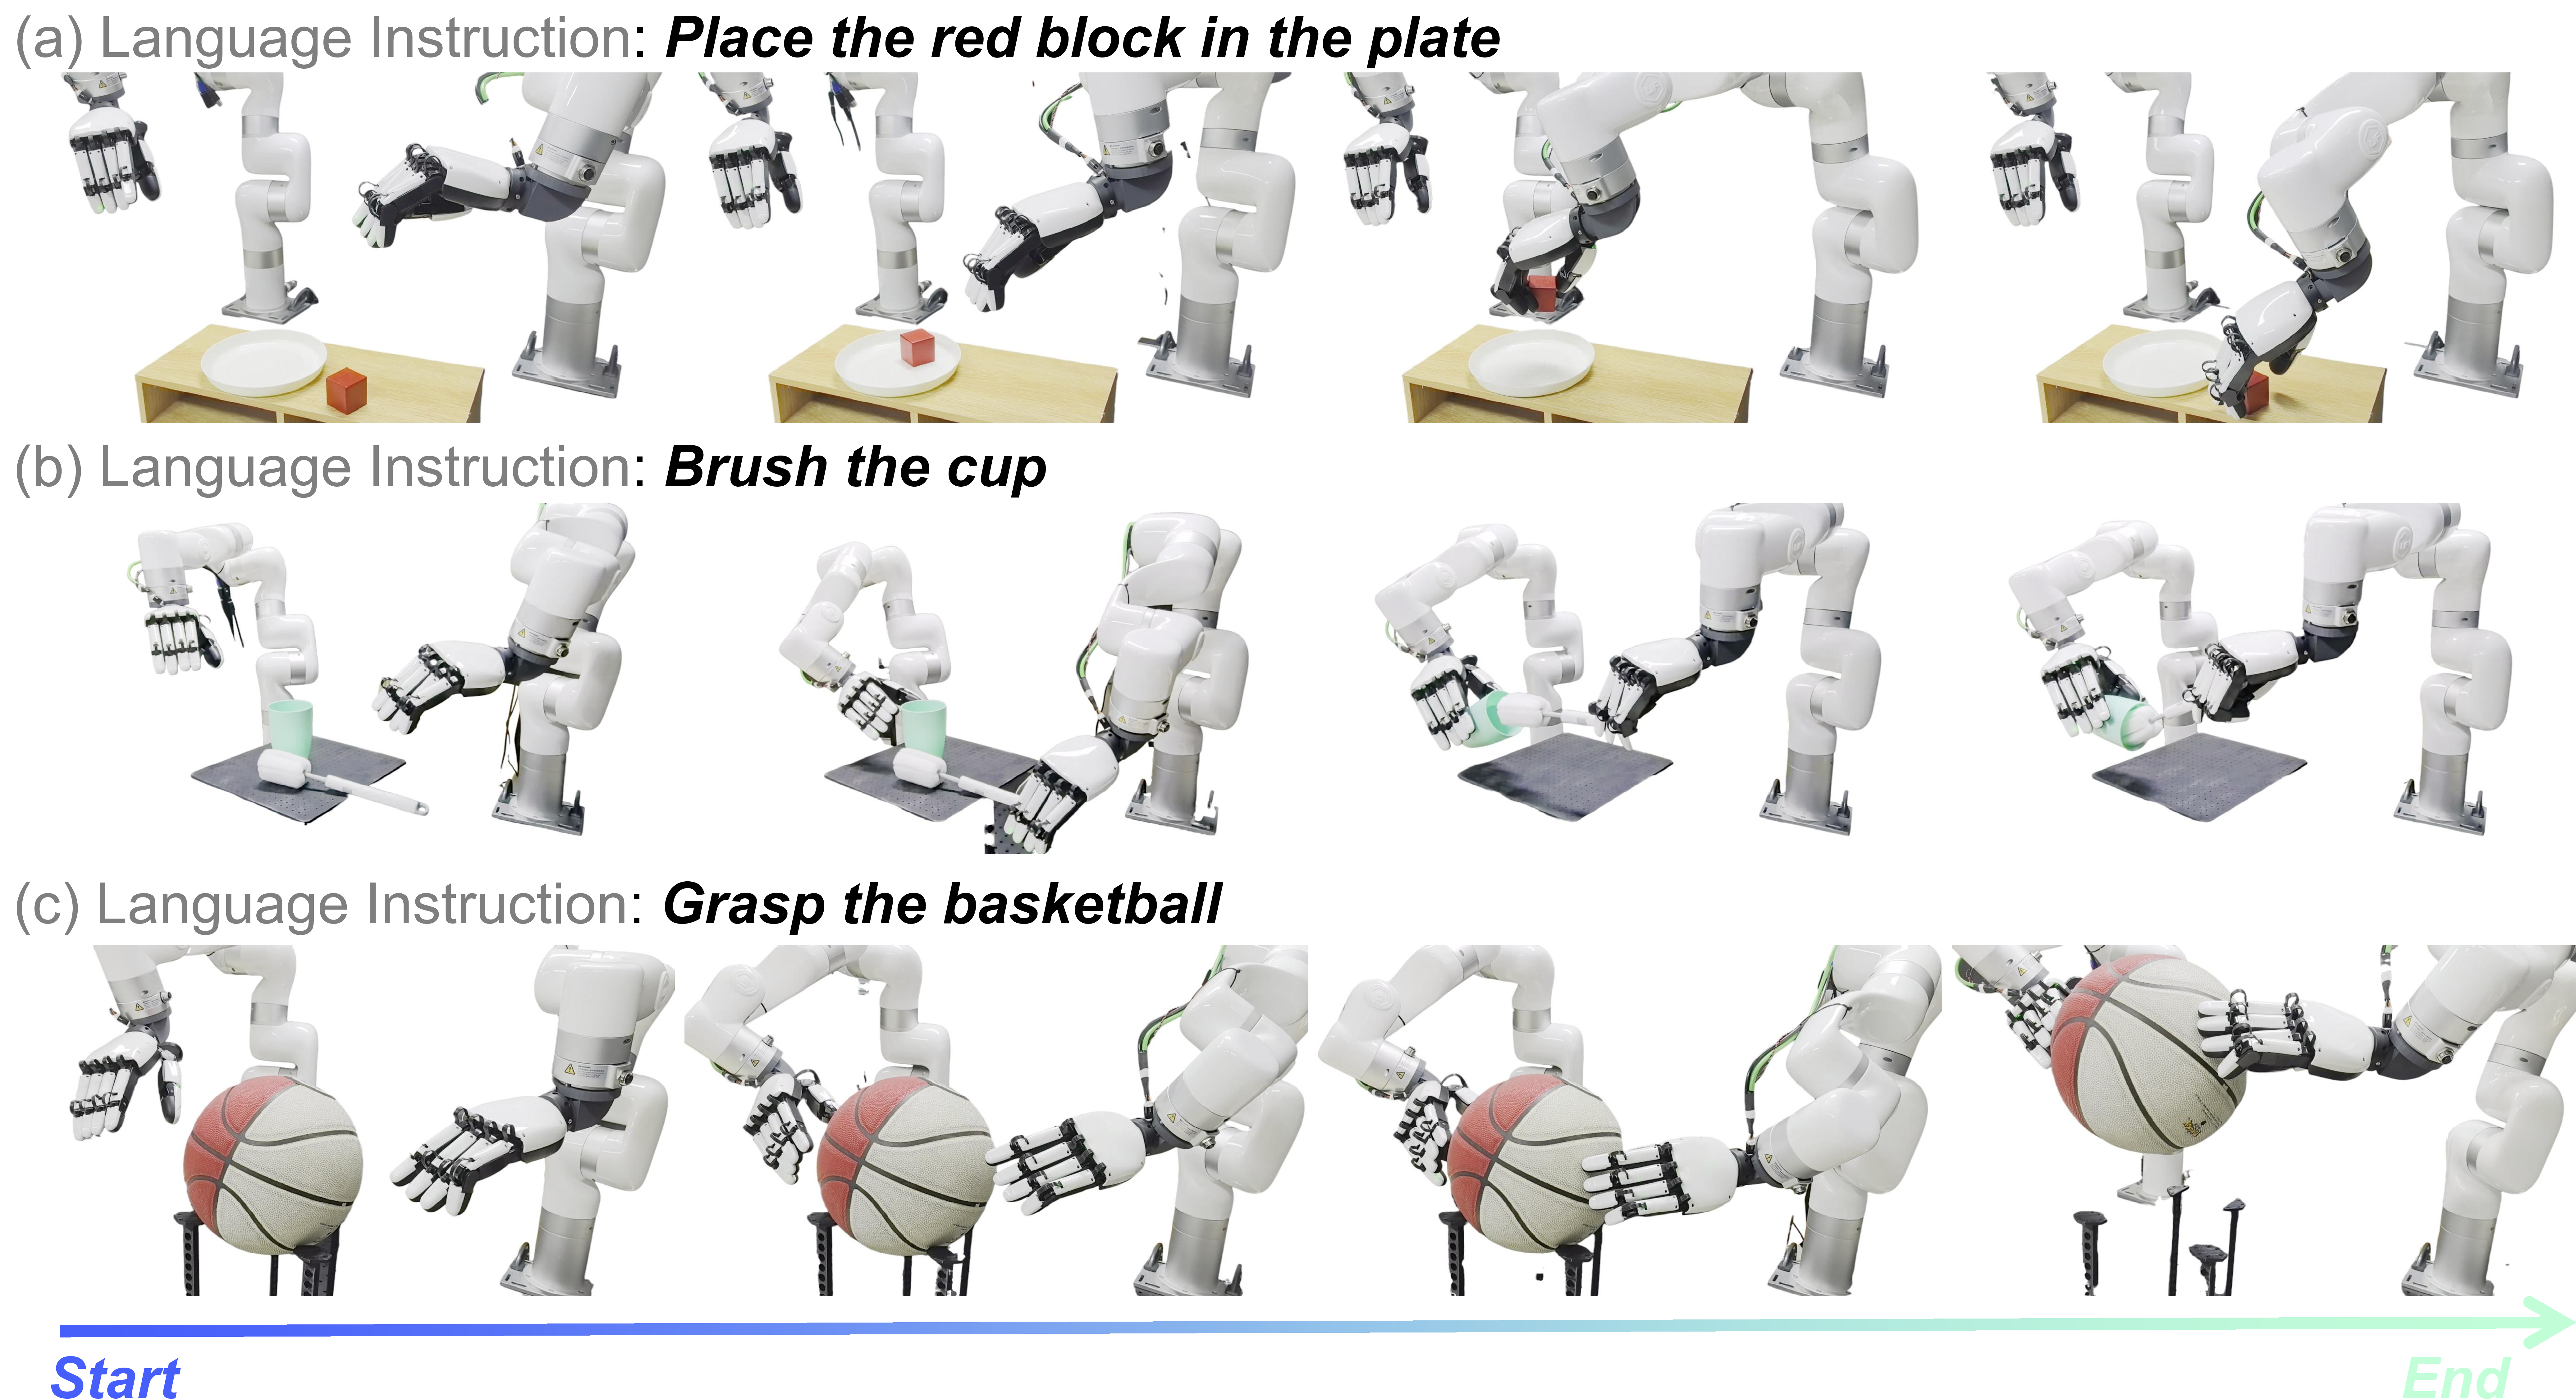
\includegraphics[width=0.96\linewidth]{pic/app_real_traj.pdf}
  % \vspace{-16pt}
  \caption{Qualitative rollouts of real-world tasks.}
  % \vspace{-16pt}
  \label{fig:app_real}
\end{figure*}




\section{Visualization of Failure Cases}

While our Structural Action Transformer (SAT) demonstrates robust performance, it is not without limitations, particularly in scenarios involving complex contact dynamics. Figure \ref{fig:failure_cases} illustrates representative failure case from our real-world experiments. Our policy is not conditioned on haptic or force-torque information. This becomes a critical bottleneck in tasks requiring precise force modulation. For example, in the ``Remove the pen cap'' task, the policy might successfully grasp the cap but fail to apply sufficient axial force to overcome the friction, resulting in the fingers slipping. These failures highlight a key avenue for future work: integrating tactile and force-sensing modalities with our structural-centric action representation.



\section{Ablation on Action Horizon Length}

In the main paper (Sec 4.3), we demonstrate that our Structural Action Transformer (SAT) is robust to the compression of the temporal trajectory, \textit{i.e.}, projecting the $T$-dimensional feature vector to a lower-dimensional embedding $d_{feat}$. Here, we provide a complementary ablation study on the original action horizon length $T$ itself.

We pre-train and fine-tune our SAT model with varying horizon lengths $T$, keeping other parameters consistent with our best model from the main paper. The average success rate on Adroitt~\cite{rajeswaran2017learning} is reported in Table~\ref{tab:app_horizon}. We observe that increasing the horizon shows a marginal decrease. The additional temporal steps appear to introduce redundancy rather than new, useful long-term information. This result validates our structural-centric approach and its inherent capacity for temporal compression. It justifies that appropriate $T$ provides a rich enough signal for compression without incurring the cost of processing unnecessary, redundant data.




\subsection{Additional Qualitative Results}

We provide additional qualitative rollouts for the real-world tasks that could not be included in the main paper due to space constraints. Figure~\ref{fig:app_real} shows rollouts for the `Brush the cup', `Grasp basketball', and `Place block in plate' real-world tasks. These visualizations highlight the policy's ability to handle complex bimanual coordination and contact-rich interactions, successfully transferring the priors learned from simulation and human data to our real-world setup.




\section{Real-World Demonstration Video}

We have included a supplementary video file  that shows our real-world experiments. The video demonstrates the performance of our SAT policy on the bimanual setup for tasks described in the main paper.


